\newpage
\setcounter{section}{0}
\renewcommand{\thesection}{\arabic{section}}

\begin{center}
    \Huge
    \textbf{Modul 2}
    
    Wireless Connection

\end{center}


\section{Pendahuluan}

Pada modul ini, kita akan membahas konfigurasi routing static dan routing dinamis pada perangkat
MikroTik. Routing merupakan proses pengiriman data antara dua atau lebih jaringan yang berbeda.

Dalam modul ini, kita akan membahas konsep dasar routing, macam-macam routing statis dan
dinamis, serta langkah-langkah untuk mengkonfigurasi kedua jenis routing ini pada perangkat
MikroTik.

Sebelum memulai pembahasan routing, penting untuk memahami konsep dasar jaringan dan
subnetting. Jaringan terdiri dari sejumlah perangkat yang terhubung satu sama lain, seperti komputer,
printer, dan perangkat jaringan lainnya. Setiap perangkat dalam jaringan memiliki alamat IP yang
unik.

Subnetting adalah proses pembagian jaringan menjadi subnet yang lebih kecil. Dengan subnetting, kita
dapat mengoptimalkan penggunaan alamat IP dan membagi jaringan menjadi beberapa segmen yang
terpisah.

Dalam routing, terdapat yang namanya protokol routing. Protokol routing adalah aturan yang
digunakan oleh perangkat jaringan untuk memilih jalur terbaik bagi pengiriman data antara jaringan
yang berbeda. Ada dua jenis protokol routing utama: routing static dan routing dinamis.

\section{Tujuan Praktikum}

Mengetahui dan memahami konfigurasi routing static dan routing dinamis pada Mikrotik.

\section{Alat dan Bahan}

Berikut adalah alat dan abhan yang digunakan:
\begin{enumerate}
    \item 2 perangkat router mikrotik.
    \item Aplikasi Winbox.
    \item 3 kabel LAN
\end{enumerate}

\section{Topologi}

berikut adalah topologi yang digunakan :

\begin{center}
    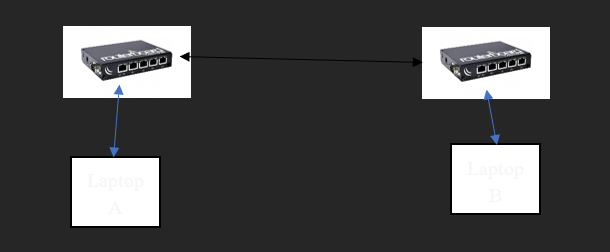
\includegraphics[width=0.7\textwidth]{image/P2/Topologi.png}    
    
    figure.1 Topologi
\end{center}


\section{Langkah Percobaan}
\begin{enumerate}
    \item Persiapan Awal
    
    \begin{enumerate}
        \item Sambungkan PC dan Router mikrotik sesuai dengan topologi
        \item Matikan Firewall pada Laptop
        \item Masuk ke aplikasi Winbox
        \item Pada bagian Neighbour, check apakah ada IP 0000 identity mikrotik
        \item Reset mikrotik ke 0000
        \item Lalu tekan connect
        
        \begin{center}
            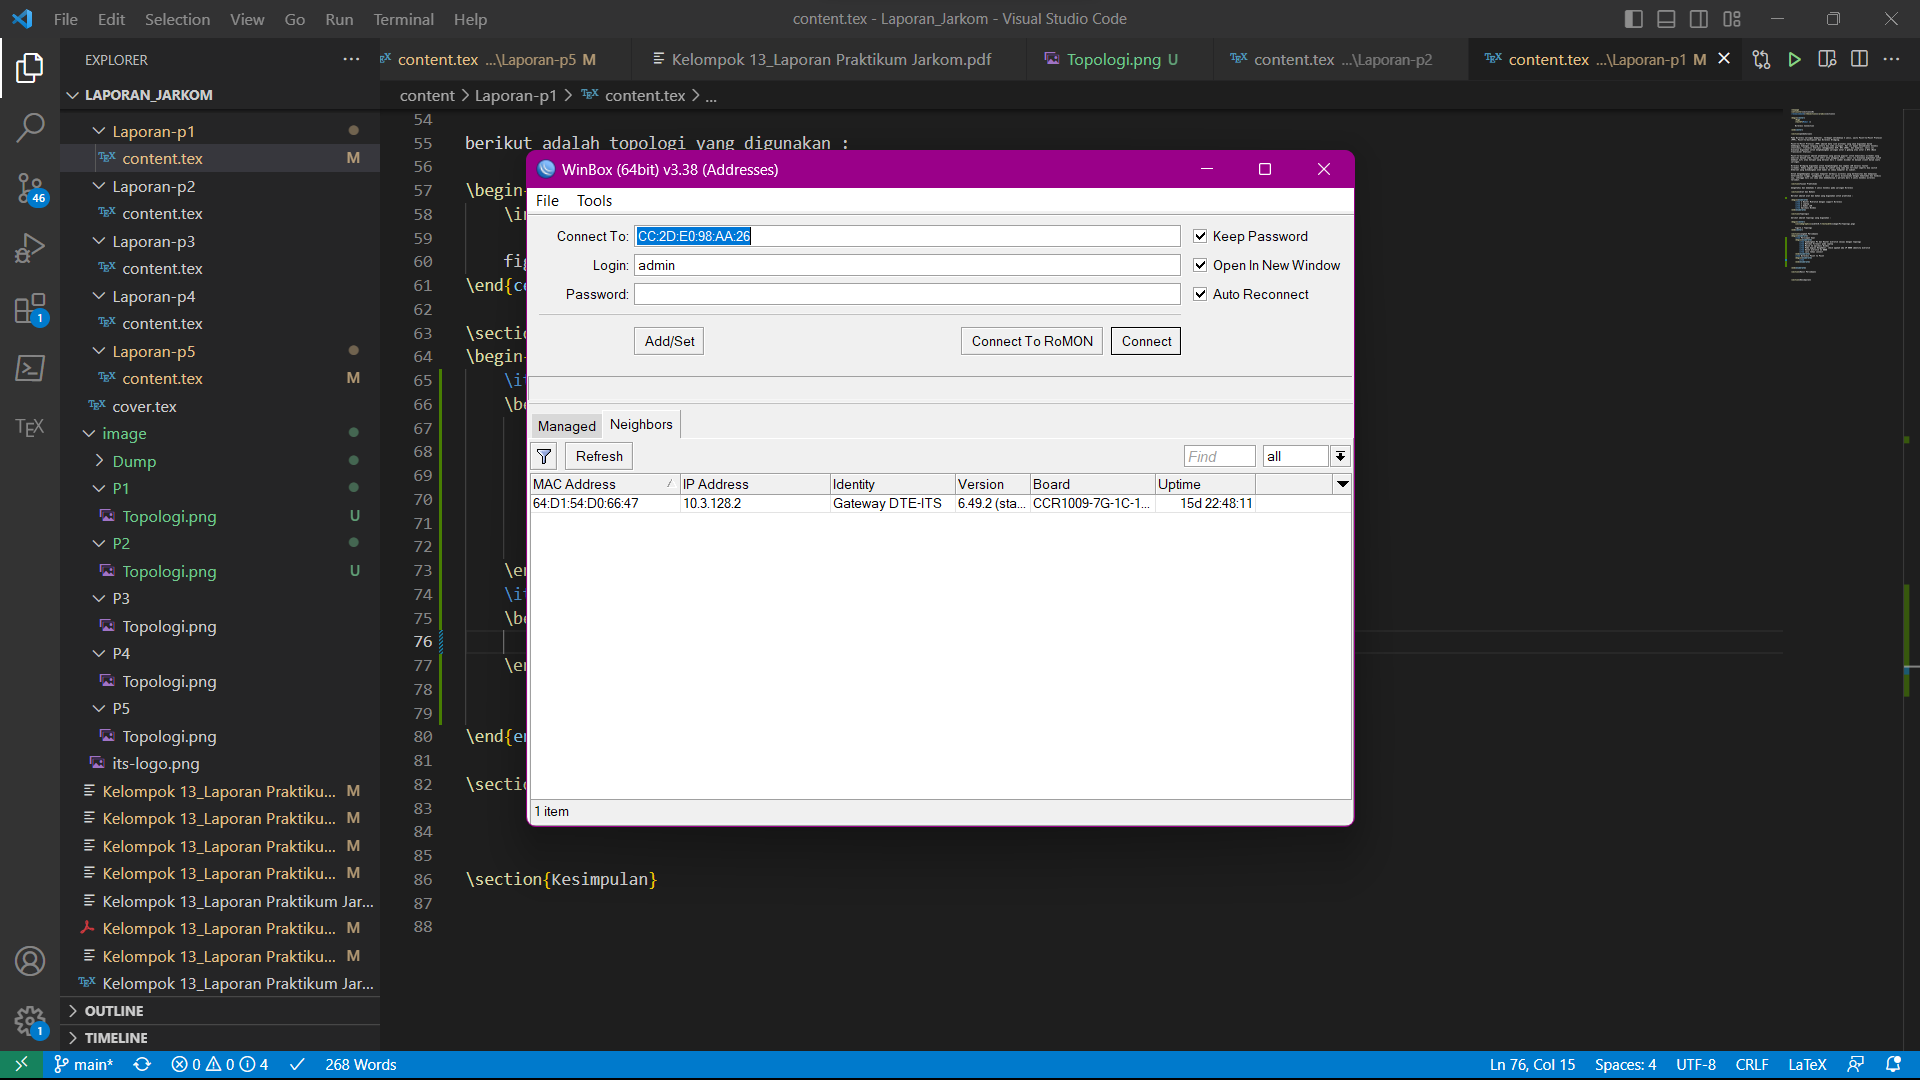
\includegraphics[width=0.7\textwidth]{image/Winbox-interface.png}    
            
            figure.2 WinBox interface
        \end{center}

    \end{enumerate}

    \item Static Routing 
    
    \begin{enumerate}
        \item Pertama lakukan konfigurasi IP address pada masing-masing router, pilih menu IP \texttt{\text>} Address \texttt{\text>} (+) \texttt{\text>} Address : (IP Address pada router) , Interface : (interface yang tersambung)
        \item Untuk melakukan routing statis, pilih menu IP \texttt{\text>} Routes \texttt{\text>} (+) \texttt{\text>} Dst . Address : (IP network client router lawan) , Gateway : (IP yang menghubungkan kedua router)
        \item Apabila sudah benar, maka akan terlihat tulisan ‘reachable’
        
        \begin{center}
            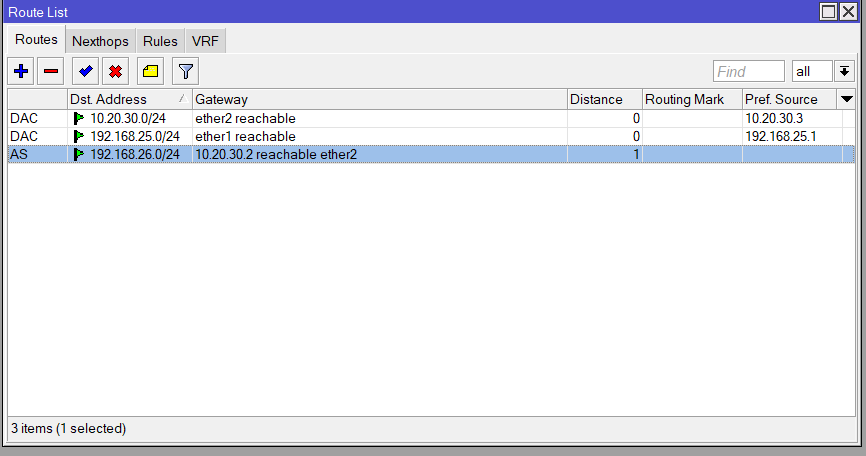
\includegraphics[width=0.7\textwidth]{image/P2/static/static-routelist.png}    
            
            figure.3 Route list
        \end{center}

        \item Setelah itu konfigurasikan DHCP servernya untuk klien yang akan terhubung, pilih menu IP \texttt{\text>} DHCP Server \texttt{\text>} (+) \texttt{\text>} DHCP Server Interface : (interface yang menghubungkan pada laptop)
        
        \begin{center}
            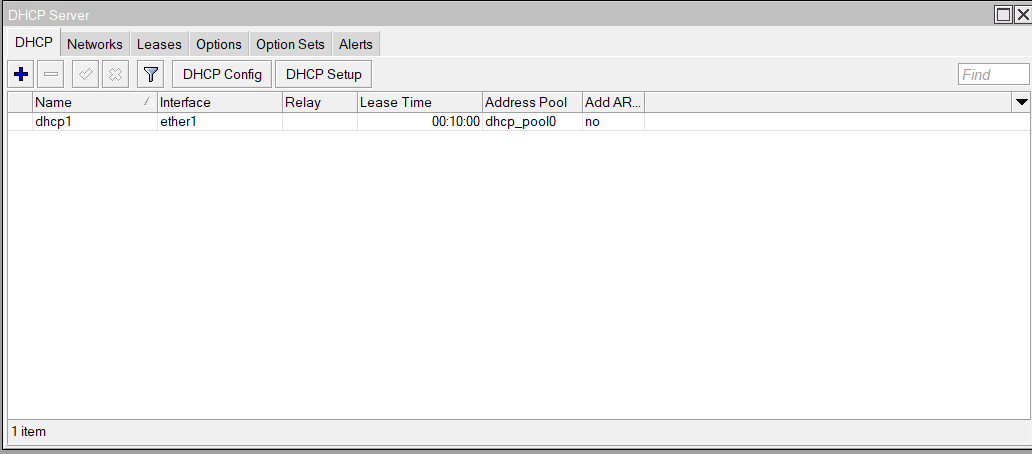
\includegraphics[width=0.7\textwidth]{image/P2/static/static-dhcpserver.png}    
            
            figure.4 DHCP Server setup
        \end{center}

        \item Static routing selesai, dapat dilakukan test ping
    \end{enumerate}
    
    \item Dynamic Routing 
    
    \begin{enumerate}
        \item Untuk melakukan routing dinamis, pilih menu Routing \texttt{\text>} RIP \texttt{\text>} Interface \texttt{\text>} (+) \texttt{\text>} Interface : (interface yang menghubungkan antar router) \texttt{\text>} Apply \texttt{\text>} OK
        \item Kemudian masih dalam window RIP, pilih tab Networks \texttt{\text>} (+) \texttt{\text>} Address : (masukan semua IP Network yang terhubung dengan router) \texttt{\text>} OK
        \item Masih dalam window RIP, pilih tab Neighbour \texttt{\text>} (+) \texttt{\text>} Address : (alamat IP router lawan)
        
        \begin{center}
            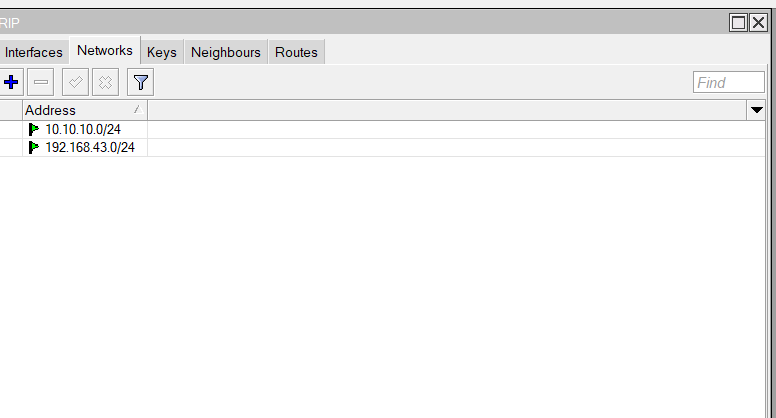
\includegraphics[width=0.7\textwidth]{image/P2/dynamic/dynamic-rip.png}    
            
            figure.5 Dynamic RIP table
        \end{center}

        \item Setelah itu lakukan konfigurasi IP pada masing-masing laptop agar sesuai dengan yang sudah terisi pada winbox
        \item Dynamic routing selesai, dapat dilakukan test ping
    \end{enumerate}
    
    
\end{enumerate}

\section{Hasil Percobaan}

\begin{enumerate}
    \item Static Routing 
    
    \begin{center}
        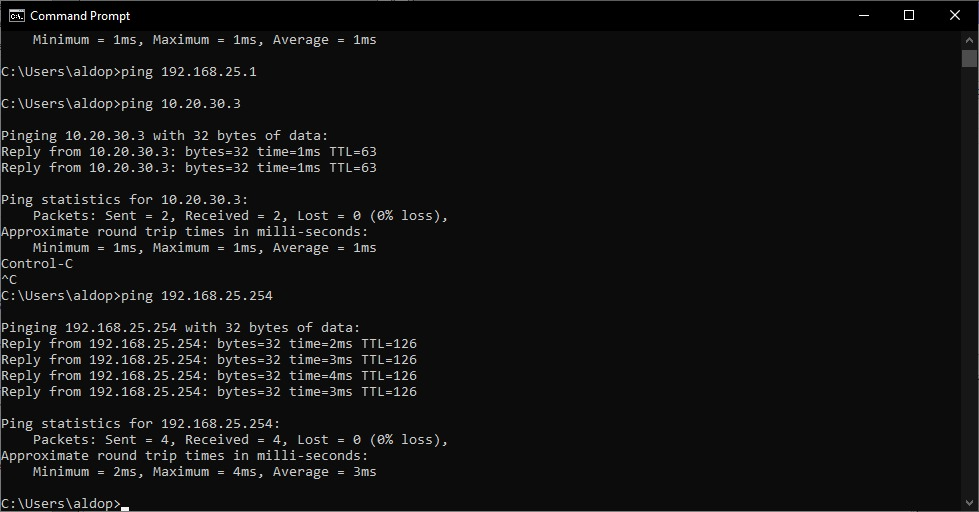
\includegraphics[width=0.7\textwidth]{image/P2/static/static-test.jpg}    
        
        figure.6 Static Routing Testing
    \end{center}

    \item Dynamic Routing 
    
    \begin{center}
        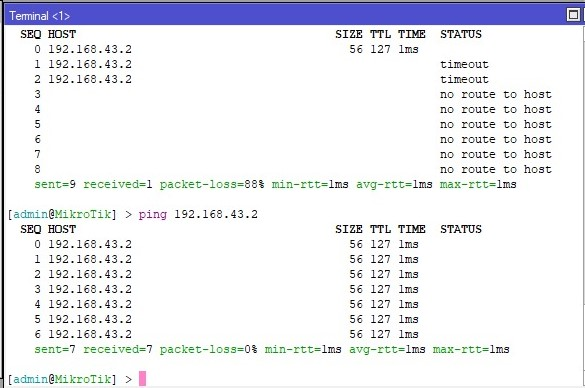
\includegraphics[width=0.7\textwidth]{image/P2/dynamic/dynamic-test.jpg}    
        
        figure.7 Dynamic Routing Testing
    \end{center}

\end{enumerate}

\section{Kesimpulan}

Static dan Dynamic Routing dapat menghubungkan komputer melalui kabel LAN 
